\documentclass{article}
\usepackage[utf8]{inputenc}
\usepackage[T1]{fontenc}
\usepackage{graphicx}
\usepackage{float}
\usepackage{hyperref}
\usepackage{listings}

\title{Ghost Hunter Simulator Report}
\author{Dylan}
\date{\today}

\begin{document}

\maketitle

\section{The Ghost Hunter Simulator}
We decided to implement in java a simulator for the whole Ghost Hunter game, a
scenario where a hunter searches for a ghost on a given graph structure. The
primary objective of this tool is to provide a framework for running
experiments to confirm or invalidate conjectures about strategies on various
types of graphs. It is important to note that while this simulator can provide
strong empirical evidence, it is not a formal proof tool. For each experiment,
the simulator calculates and outputs the average number of rounds required for
the hunter to find the ghost.

\subsection{Core Concepts}
As described before, the game is played on a graph. A ghost hides on one of the 
vertices, and a hunter attempts to find it. The simulation revolves around the
hunter's strategy for choosing which vertex to inspect in each round. The
efficiency of a strategy is measured by the number of rounds it takes to
capture the ghost.

\subsection{Configuration}
All simulation parameters are managed through a single configuration file named 
\texttt{config.toml}. This file allows users to define the specifics of the
experiment they wish to run without modifying the source code. The main
configurable parameters are detailed below.

\subsubsection{Execution Parameters}
\begin{itemize}
    \item \texttt{nbSimu}: Defines the number of times each simulation is
    repeated. A higher number provides a more accurate average of the number of 
    rounds needed to win.
    \item \texttt{policy}: Determines the hunter's strategy.
    \begin{itemize}
        \item \texttt{RANDOM}: The hunter chooses a random vertex at each round,
        excluding the one just visited. (Works on any \texttt{graphType} and
        any \texttt{execType}).
        \item \texttt{HIGH\_DEGREE\_PRIO}: The hunter randomly chooses a vertex,
        with a bias towards vertices with a higher degree, excluding the one
        just visited. (Works on any \texttt{graphType} and any
        \texttt{execType}).
        \item \texttt{NEXT\_VERTEX}: A deterministic strategy for cycle graphs
        where the hunter moves to the next adjacent vertex. (Works on
        \texttt{graphType} = \texttt{N\_CYCLE}).
    \end{itemize}
    \item \texttt{execType}: Specifies the mode of execution.
    \begin{itemize}
        \item \texttt{SINGLE}: Runs the simulation on a single, specified graph.
        (Works on \texttt{graphType} = \texttt{N\_CYCLE}, \texttt{N\_COMP} and
        \texttt{FROM\_FILE}).
        \item \texttt{UP\_TO\_SIZE}: Runs simulations on a series of graphs of
        a specific type, from size 3 up to a defined maximum size \texttt{N}.
        (Works on \texttt{graphType} = \texttt{N\_CYCLE}, \texttt{N\_COMP}).
        \item \texttt{FAMILY}: Runs simulations for a family of graphs,
        particularly useful for k-regular graphs. (Works on any
        \texttt{graphType} but most interesting with \texttt{N\_K\_REGULAR}).
    \end{itemize}
\end{itemize}

\subsubsection{Graph Parameters}
\begin{itemize}
    \item \texttt{graphType}: The type of graph to be used in the simulation.
    \begin{itemize}
        \item \texttt{N\_CYCLE}: A cycle graph with N vertices.
        \item \texttt{N\_COMP}: A complete graph with N vertices.
        \item \texttt{N\_K\_REGULAR}: A k-regular graph with N vertices.
        \item \texttt{N\_CONN}: A random connected graph with N vertices.
        \item \texttt{FROM\_FILE}: A graph loaded from a user-provided file.
    \end{itemize}
    
    Below are visual representations for each graph type:

    \begin{figure}[H]
        \centering
        \begin{minipage}{0.45\textwidth}
            \centering
            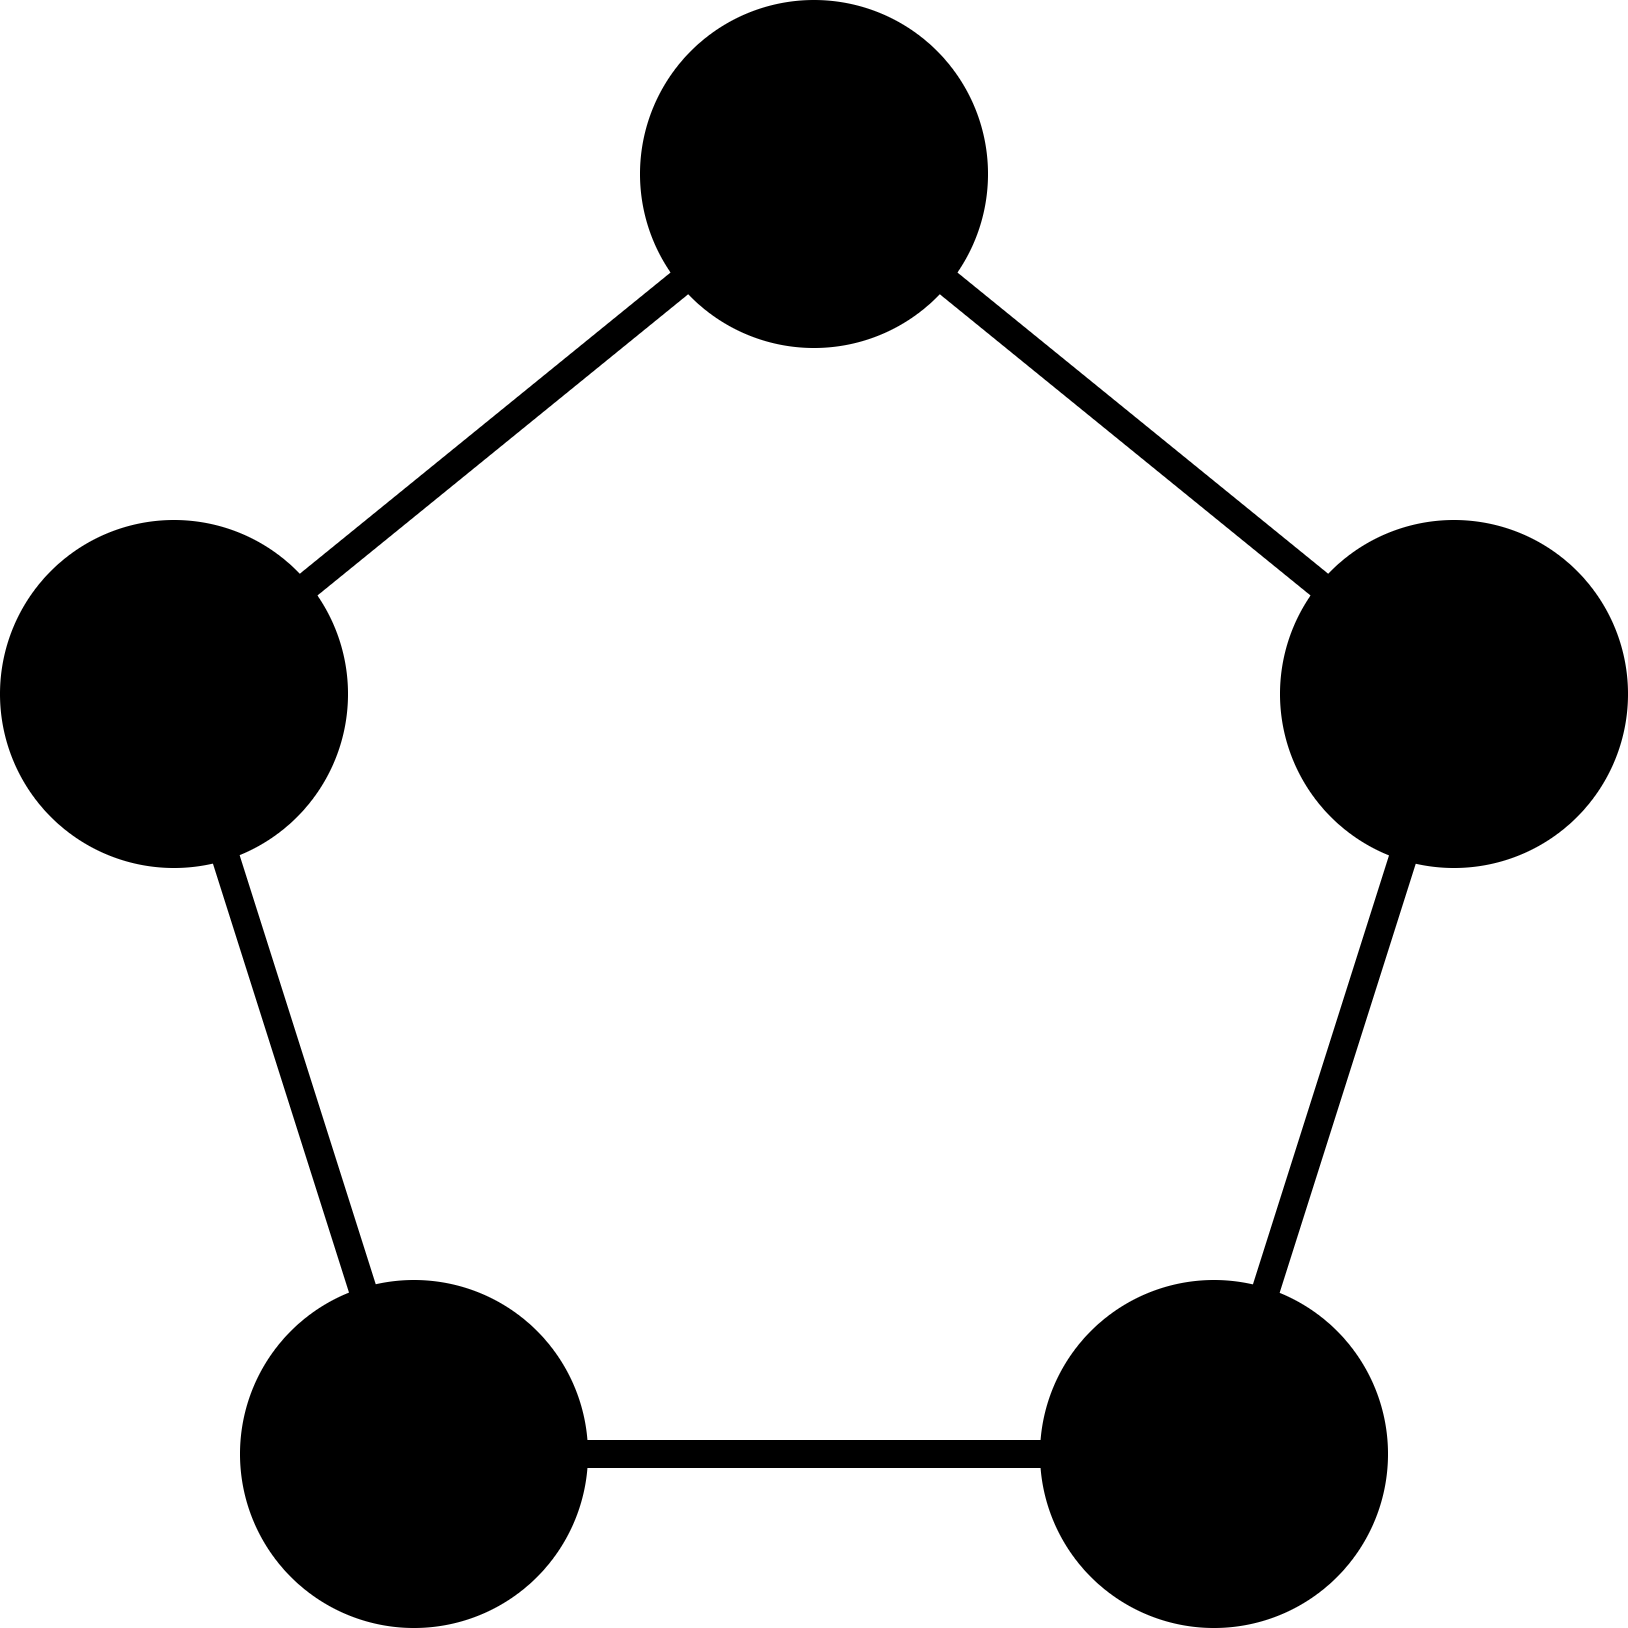
\includegraphics[width=\linewidth]{images/black_5_cycle.png}
            \caption{A 5-vertex cycle graph (\texttt{N\_CYCLE}).}
        \end{minipage}\hfill
        \begin{minipage}{0.45\textwidth}
            \centering
            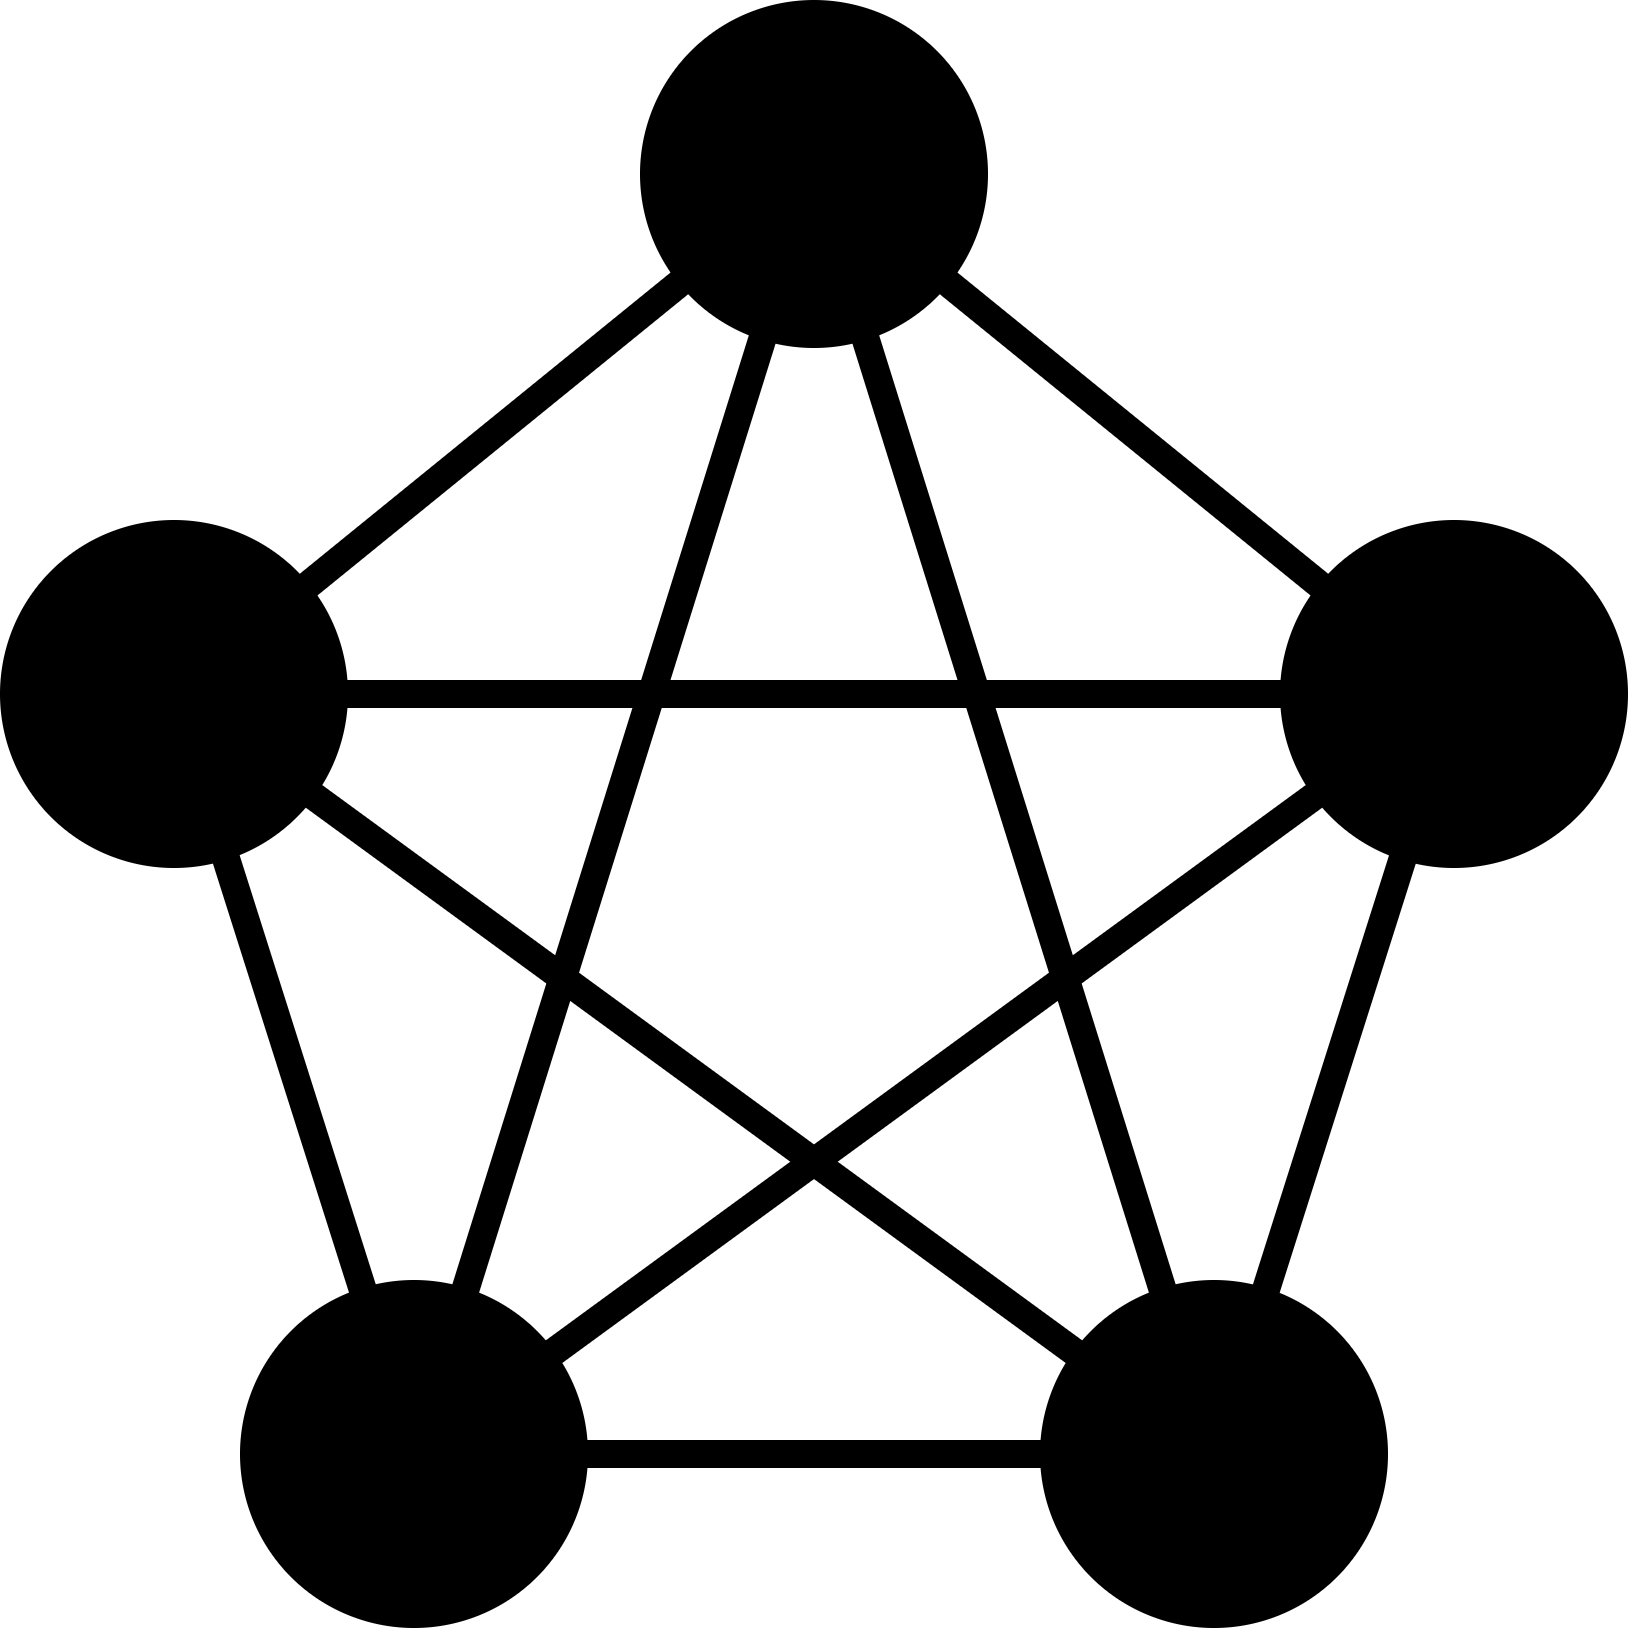
\includegraphics[width=\linewidth]{images/black_5_comp.png}
            \caption{A 5-vertex complete graph (\texttt{N\_COMP}).}
        \end{minipage}
    \end{figure}

    \begin{figure}[H]
        \centering
        \begin{minipage}{0.45\textwidth}
            \centering
            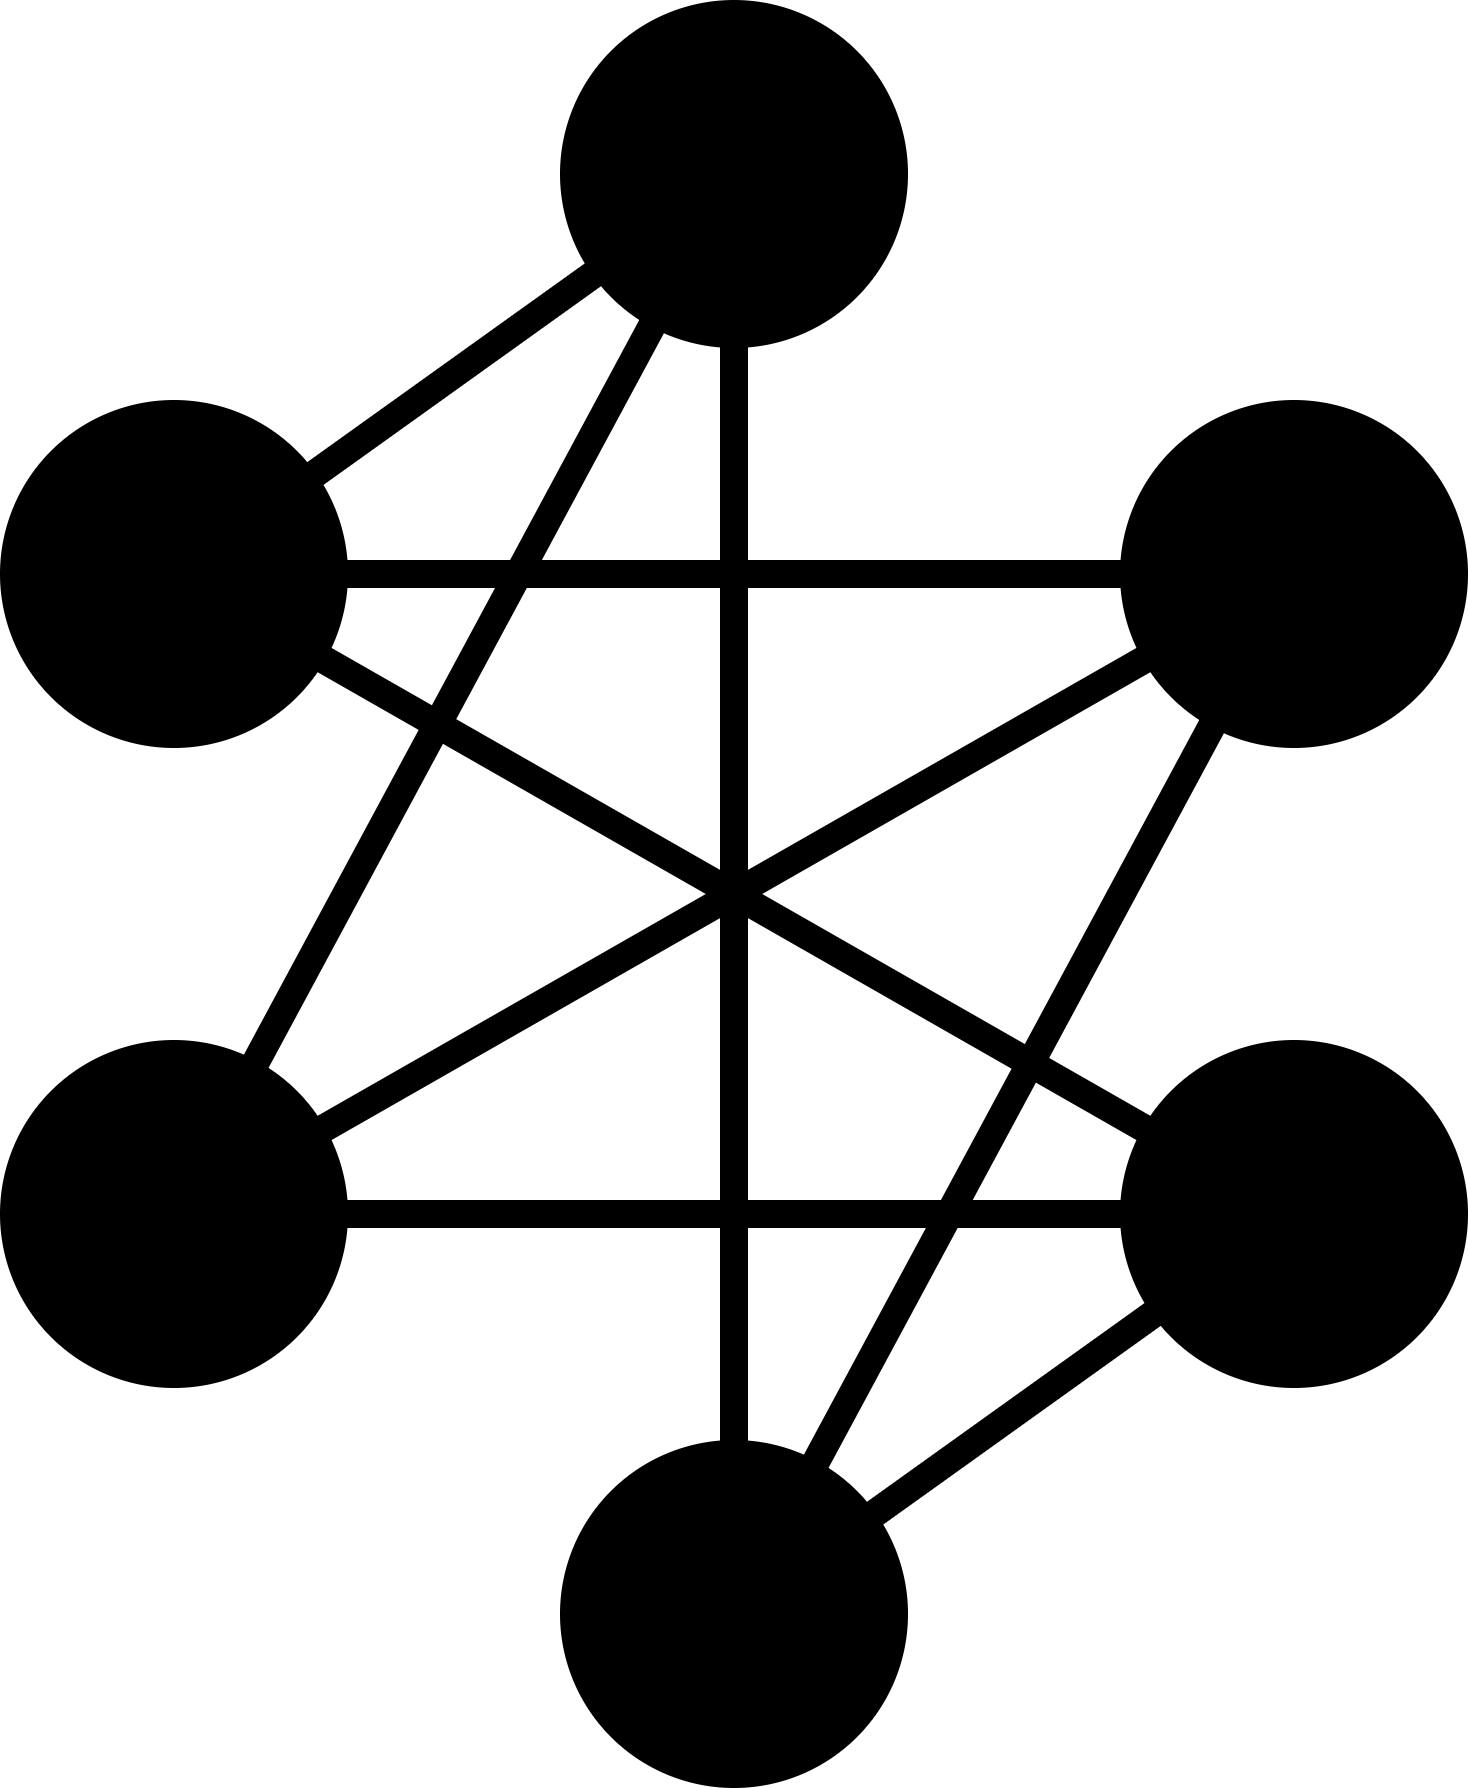
\includegraphics[width=\linewidth]{images/black_6_3_regular.png}
            \caption{A 6-vertex 3-regular graph (\texttt{N\_K\_REGULAR}).}
        \end{minipage}\hfill
        \begin{minipage}{0.45\textwidth}
            \centering
            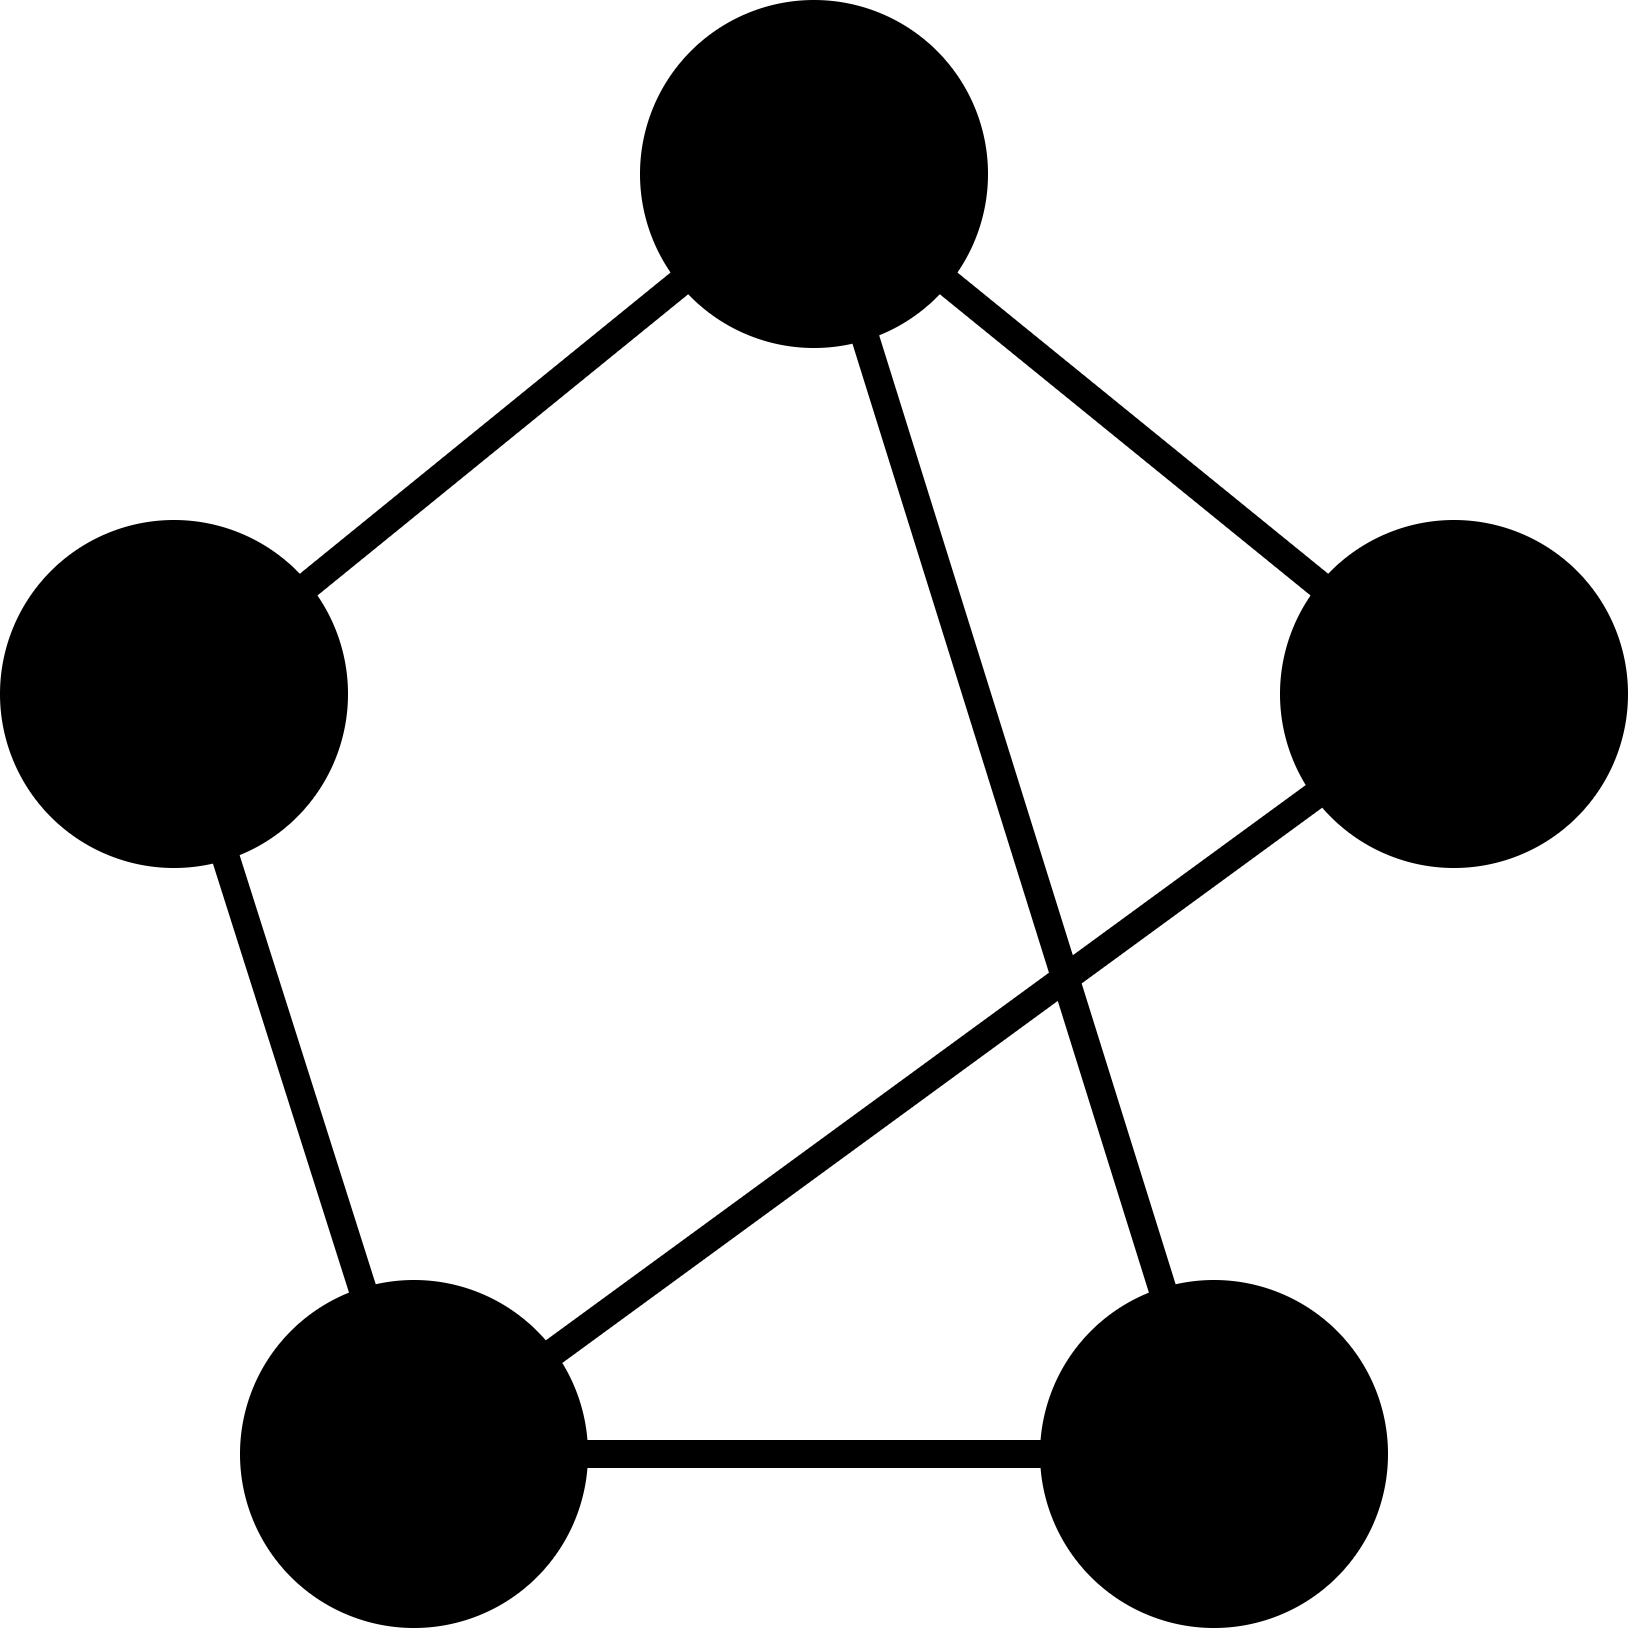
\includegraphics[width=\linewidth]{images/black_5_conn.png}
            \caption{A 5-vertex connected graph (\texttt{N\_CONN}).}
        \end{minipage}
    \end{figure}
    
    For the \texttt{FROM\_FILE} type, the graph is defined by its adjacency
    matrix in a text file, as shown in this example of a 7-cycle:
    \begin{verbatim}
7
0 1 0 0 0 0 1
1 0 1 0 0 0 0
0 1 0 1 0 0 0
0 0 1 0 1 0 0
0 0 0 1 0 1 0
0 0 0 0 1 0 1
1 0 0 0 0 1 0
    \end{verbatim}
    
    \item \texttt{filename}: The path to the file describing the graph when
    \texttt{graphType} is set to \texttt{FROM\_FILE}. (Works with any
    \texttt{graphType} but ignored if not \texttt{FROM\_FILE}).
    \item \texttt{N}: The number of vertices in the graph. For
    \texttt{UP\_TO\_SIZE} execution, this is the maximum size. (Works with any
    \texttt{graphType} but ignored if \texttt{FROM\_FILE}).
    \item \texttt{K}: The degree of each vertex for a k-regular graph. (Works
    with any \texttt{graphType} but ignored if not \texttt{N\_K\_REGULAR}).
\end{itemize}

\subsection{Output}
The primary output of the simulator is the average number of rounds required to 
complete the game for a given configuration. This statistical result, averaged
over \texttt{nbSimu} runs, helps in comparing the effectiveness of different
hunting strategies on various graph structures.

\end{document}
